\documentclass[]{article}
\usepackage{lmodern}
\usepackage{amssymb,amsmath}
\usepackage{ifxetex,ifluatex}
\usepackage{fixltx2e} % provides \textsubscript
\ifnum 0\ifxetex 1\fi\ifluatex 1\fi=0 % if pdftex
  \usepackage[T1]{fontenc}
  \usepackage[utf8]{inputenc}
\else % if luatex or xelatex
  \ifxetex
    \usepackage{mathspec}
  \else
    \usepackage{fontspec}
  \fi
  \defaultfontfeatures{Ligatures=TeX,Scale=MatchLowercase}
\fi
% use upquote if available, for straight quotes in verbatim environments
\IfFileExists{upquote.sty}{\usepackage{upquote}}{}
% use microtype if available
\IfFileExists{microtype.sty}{%
\usepackage{microtype}
\UseMicrotypeSet[protrusion]{basicmath} % disable protrusion for tt fonts
}{}
\usepackage[margin=1in]{geometry}
\usepackage{hyperref}
\hypersetup{unicode=true,
            pdftitle={Course Project 2},
            pdfauthor={Joseph Audras and Devin Romines},
            pdfborder={0 0 0},
            breaklinks=true}
\urlstyle{same}  % don't use monospace font for urls
\usepackage{color}
\usepackage{fancyvrb}
\newcommand{\VerbBar}{|}
\newcommand{\VERB}{\Verb[commandchars=\\\{\}]}
\DefineVerbatimEnvironment{Highlighting}{Verbatim}{commandchars=\\\{\}}
% Add ',fontsize=\small' for more characters per line
\usepackage{framed}
\definecolor{shadecolor}{RGB}{248,248,248}
\newenvironment{Shaded}{\begin{snugshade}}{\end{snugshade}}
\newcommand{\AlertTok}[1]{\textcolor[rgb]{0.94,0.16,0.16}{#1}}
\newcommand{\AnnotationTok}[1]{\textcolor[rgb]{0.56,0.35,0.01}{\textbf{\textit{#1}}}}
\newcommand{\AttributeTok}[1]{\textcolor[rgb]{0.77,0.63,0.00}{#1}}
\newcommand{\BaseNTok}[1]{\textcolor[rgb]{0.00,0.00,0.81}{#1}}
\newcommand{\BuiltInTok}[1]{#1}
\newcommand{\CharTok}[1]{\textcolor[rgb]{0.31,0.60,0.02}{#1}}
\newcommand{\CommentTok}[1]{\textcolor[rgb]{0.56,0.35,0.01}{\textit{#1}}}
\newcommand{\CommentVarTok}[1]{\textcolor[rgb]{0.56,0.35,0.01}{\textbf{\textit{#1}}}}
\newcommand{\ConstantTok}[1]{\textcolor[rgb]{0.00,0.00,0.00}{#1}}
\newcommand{\ControlFlowTok}[1]{\textcolor[rgb]{0.13,0.29,0.53}{\textbf{#1}}}
\newcommand{\DataTypeTok}[1]{\textcolor[rgb]{0.13,0.29,0.53}{#1}}
\newcommand{\DecValTok}[1]{\textcolor[rgb]{0.00,0.00,0.81}{#1}}
\newcommand{\DocumentationTok}[1]{\textcolor[rgb]{0.56,0.35,0.01}{\textbf{\textit{#1}}}}
\newcommand{\ErrorTok}[1]{\textcolor[rgb]{0.64,0.00,0.00}{\textbf{#1}}}
\newcommand{\ExtensionTok}[1]{#1}
\newcommand{\FloatTok}[1]{\textcolor[rgb]{0.00,0.00,0.81}{#1}}
\newcommand{\FunctionTok}[1]{\textcolor[rgb]{0.00,0.00,0.00}{#1}}
\newcommand{\ImportTok}[1]{#1}
\newcommand{\InformationTok}[1]{\textcolor[rgb]{0.56,0.35,0.01}{\textbf{\textit{#1}}}}
\newcommand{\KeywordTok}[1]{\textcolor[rgb]{0.13,0.29,0.53}{\textbf{#1}}}
\newcommand{\NormalTok}[1]{#1}
\newcommand{\OperatorTok}[1]{\textcolor[rgb]{0.81,0.36,0.00}{\textbf{#1}}}
\newcommand{\OtherTok}[1]{\textcolor[rgb]{0.56,0.35,0.01}{#1}}
\newcommand{\PreprocessorTok}[1]{\textcolor[rgb]{0.56,0.35,0.01}{\textit{#1}}}
\newcommand{\RegionMarkerTok}[1]{#1}
\newcommand{\SpecialCharTok}[1]{\textcolor[rgb]{0.00,0.00,0.00}{#1}}
\newcommand{\SpecialStringTok}[1]{\textcolor[rgb]{0.31,0.60,0.02}{#1}}
\newcommand{\StringTok}[1]{\textcolor[rgb]{0.31,0.60,0.02}{#1}}
\newcommand{\VariableTok}[1]{\textcolor[rgb]{0.00,0.00,0.00}{#1}}
\newcommand{\VerbatimStringTok}[1]{\textcolor[rgb]{0.31,0.60,0.02}{#1}}
\newcommand{\WarningTok}[1]{\textcolor[rgb]{0.56,0.35,0.01}{\textbf{\textit{#1}}}}
\usepackage{graphicx,grffile}
\makeatletter
\def\maxwidth{\ifdim\Gin@nat@width>\linewidth\linewidth\else\Gin@nat@width\fi}
\def\maxheight{\ifdim\Gin@nat@height>\textheight\textheight\else\Gin@nat@height\fi}
\makeatother
% Scale images if necessary, so that they will not overflow the page
% margins by default, and it is still possible to overwrite the defaults
% using explicit options in \includegraphics[width, height, ...]{}
\setkeys{Gin}{width=\maxwidth,height=\maxheight,keepaspectratio}
\IfFileExists{parskip.sty}{%
\usepackage{parskip}
}{% else
\setlength{\parindent}{0pt}
\setlength{\parskip}{6pt plus 2pt minus 1pt}
}
\setlength{\emergencystretch}{3em}  % prevent overfull lines
\providecommand{\tightlist}{%
  \setlength{\itemsep}{0pt}\setlength{\parskip}{0pt}}
\setcounter{secnumdepth}{0}
% Redefines (sub)paragraphs to behave more like sections
\ifx\paragraph\undefined\else
\let\oldparagraph\paragraph
\renewcommand{\paragraph}[1]{\oldparagraph{#1}\mbox{}}
\fi
\ifx\subparagraph\undefined\else
\let\oldsubparagraph\subparagraph
\renewcommand{\subparagraph}[1]{\oldsubparagraph{#1}\mbox{}}
\fi

%%% Use protect on footnotes to avoid problems with footnotes in titles
\let\rmarkdownfootnote\footnote%
\def\footnote{\protect\rmarkdownfootnote}

%%% Change title format to be more compact
\usepackage{titling}

% Create subtitle command for use in maketitle
\providecommand{\subtitle}[1]{
  \posttitle{
    \begin{center}\large#1\end{center}
    }
}

\setlength{\droptitle}{-2em}

  \title{Course Project 2}
    \pretitle{\vspace{\droptitle}\centering\huge}
  \posttitle{\par}
    \author{Joseph Audras and Devin Romines}
    \preauthor{\centering\large\emph}
  \postauthor{\par}
      \predate{\centering\large\emph}
  \postdate{\par}
    \date{May 13, 2019}


\begin{document}
\maketitle

\hypertarget{introduction}{%
\section{Introduction}\label{introduction}}

Dataset Source:
\url{https://www.kaggle.com/lava18/google-play-store-apps}

\hypertarget{description}{%
\subsection{Description}\label{description}}

The Google Play Store Data Set is a data set containing data on over
10,000 apps in the Google Play Store for Android products. The data set
looks at things such as rating, number of installations, and genre to
produce a plethora of information on each app. For this project, we
would like to see if the rating of the app can be accurately predicted
by the variables provided in the data set.

The data set was gathered from
\url{https://www.kaggle.com/lava18/google-play-store-apps} which was
last updated 2 months ago, giving us Version 6, with which we are
working. The data was posted by Lavanya Gupta, a software engineer at
HSBC Software Development in India. More information on her can be found
here \url{https://www.kaggle.com/lava18}. The information in the data
set was scraped from the Google Play Store by Lavanya Gupta, in an
effort to provide similar information on its apps as is publically
available from the Apple App Store so that developers may be more
inclined to work in the Android market.

\begin{Shaded}
\begin{Highlighting}[]
\KeywordTok{library}\NormalTok{(tidyverse)}
\KeywordTok{library}\NormalTok{(lubridate)}
\KeywordTok{library}\NormalTok{(ggplot2)}
\end{Highlighting}
\end{Shaded}

\hypertarget{data-dictionary}{%
\section{Data Dictionary}\label{data-dictionary}}

\begin{itemize}
\item
  App -- Factor, 9660 levels -- The name of the app.
\item
  Category -- Factor, 34 levels -- The general type of app, such as
  Dating, Cooking, or Art and Design
\item
  Rating -- Numerical, range from 0-5 -- The rating of the app on a
  scale from 0-5.
\item
  Reviews -- Number, very wide range -- The number of reviews that the
  app received.
\item
  Size (Removed in Cleaning) -- Factor, 462 levels -- The size in
  megabytes of the app.
\item
  Installs -- Number, given as a factor of 10 -- The number of
  installations an app received.
\item
  Type (Removed in Cleaning) -- Factor, 4 levels -- Whether or not the
  app is free.
\item
  Price -- Number, mostly 0 but some go very high -- The Price of the
  app.
\item
  Content.Rating -- Factor, 4 levels -- The rating for the app,
  Everyone, Everyone 10+, Mature 17+, and Teen.
\item
  Genres -- Factor, 120 levels -- The genre of the app, Action, Action
  and Adventure, etc.
\item
  Last.Updated -- Factor, 1378 levels -- The date on which the app was
  last updated, given in multiple formats.
\item
  Current.Ver (Removed in Cleaning) -- Factor, 2834 levels -- The
  current version of the app, 0.0.0.2, 0.0.1, etc.
\item
  Android.Ver (Removed in Cleaning) -- Factor, 35 levels -- The version
  of Android phone required to use the app, given in the form, ``version
  and up''
\end{itemize}

\hypertarget{data-cleaning}{%
\section{Data Cleaning}\label{data-cleaning}}

Here we load the data set.

\begin{Shaded}
\begin{Highlighting}[]
\NormalTok{RawData <-}\StringTok{ }\KeywordTok{read.csv}\NormalTok{(}\StringTok{"googleplaystore.csv"}\NormalTok{)}
\end{Highlighting}
\end{Shaded}

This next code removes a problematic row that we found to have severe
errors when it was inputed.

\begin{Shaded}
\begin{Highlighting}[]
\NormalTok{GooglePlayStore <-}\StringTok{ }\NormalTok{RawData[}\OperatorTok{-}\KeywordTok{c}\NormalTok{(}\DecValTok{10473}\NormalTok{), ]}
\end{Highlighting}
\end{Shaded}

Some of the values in the data set for the Rating value, which is the
one we are looking at, read as NaN, so we will remove all entries that
contain that value.

\begin{Shaded}
\begin{Highlighting}[]
\NormalTok{GooglePlayStore <-}\StringTok{ }\NormalTok{GooglePlayStore[}\OperatorTok{-}\KeywordTok{grep}\NormalTok{(}\StringTok{"NaN"}\NormalTok{, GooglePlayStore}\OperatorTok{$}\NormalTok{Rating), ]}
\end{Highlighting}
\end{Shaded}

The Reviews variable was initially given as a factor variable. Here we
change that to be a numeric as it should be.

\begin{Shaded}
\begin{Highlighting}[]
\NormalTok{GooglePlayStore}\OperatorTok{$}\NormalTok{Reviews <-}\StringTok{ }\KeywordTok{as.numeric}\NormalTok{(}\KeywordTok{as.character}\NormalTok{(GooglePlayStore}\OperatorTok{$}\NormalTok{Reviews))}
\end{Highlighting}
\end{Shaded}

The size variable was deemed unnecessary for our goals for this project
so here we remove it.

\begin{Shaded}
\begin{Highlighting}[]
\NormalTok{GooglePlayStore <-}\StringTok{ }\NormalTok{GooglePlayStore[, }\DecValTok{-5}\NormalTok{]}
\end{Highlighting}
\end{Shaded}

The Installs variable was initially given as a factor, with undesirable
formatting. Here we remove the characters in the entries we do not want
and then convert the Installs variable to a numeric as desired.

\begin{Shaded}
\begin{Highlighting}[]
\NormalTok{GooglePlayStore}\OperatorTok{$}\NormalTok{Installs <-}\StringTok{ }\KeywordTok{gsub}\NormalTok{(}\StringTok{"}\CharTok{\textbackslash{}\textbackslash{}}\StringTok{D"}\NormalTok{, }\StringTok{""}\NormalTok{, GooglePlayStore}\OperatorTok{$}\NormalTok{Installs)}
\NormalTok{GooglePlayStore}\OperatorTok{$}\NormalTok{Installs <-}\StringTok{ }\KeywordTok{as.numeric}\NormalTok{(}\KeywordTok{as.character}\NormalTok{(GooglePlayStore}\OperatorTok{$}\NormalTok{Installs))}
\end{Highlighting}
\end{Shaded}

The Type variable merely indicates whether or not the app is free, which
is also given by the better variable, Price, so here we remove it.

\begin{Shaded}
\begin{Highlighting}[]
\NormalTok{GooglePlayStore <-}\StringTok{ }\NormalTok{GooglePlayStore[, }\DecValTok{-6}\NormalTok{]}
\end{Highlighting}
\end{Shaded}

The Price variable is interesting, here we had to remove the dollar sign
as we wanted to convert it to a numeric variable; however, when removing
the dollar sign we also noticed that the code also removed the decimal
point. To recover it, we simply divided every price by 100. This solved
the problem.

\begin{Shaded}
\begin{Highlighting}[]
\NormalTok{GooglePlayStore}\OperatorTok{$}\NormalTok{Price <-}\StringTok{ }\KeywordTok{gsub}\NormalTok{(}\StringTok{"[[:punct:]]"}\NormalTok{, }\StringTok{""}\NormalTok{, GooglePlayStore}\OperatorTok{$}\NormalTok{Price)}
\NormalTok{GooglePlayStore}\OperatorTok{$}\NormalTok{Price <-}\StringTok{ }\KeywordTok{as.numeric}\NormalTok{(GooglePlayStore}\OperatorTok{$}\NormalTok{Price)}
\NormalTok{GooglePlayStore}\OperatorTok{$}\NormalTok{Price <-}\StringTok{ }\NormalTok{GooglePlayStore}\OperatorTok{$}\NormalTok{Price}\OperatorTok{/}\DecValTok{100}
\end{Highlighting}
\end{Shaded}

We determined that the Current.Ver variable was irrelevant to our goals,
so here we remove it.

\begin{Shaded}
\begin{Highlighting}[]
\NormalTok{GooglePlayStore <-}\StringTok{ }\NormalTok{GooglePlayStore[, }\DecValTok{-10}\NormalTok{]}
\end{Highlighting}
\end{Shaded}

We also determined that the Android.Ver variable was irrelevant to our
goals, so here we remove that as well.

\begin{Shaded}
\begin{Highlighting}[]
\NormalTok{GooglePlayStore <-}\StringTok{ }\NormalTok{GooglePlayStore[, }\DecValTok{-10}\NormalTok{]}
\end{Highlighting}
\end{Shaded}

Here we write the cleaned data set to disk.

\begin{Shaded}
\begin{Highlighting}[]
\KeywordTok{write.csv}\NormalTok{(GooglePlayStore,}\StringTok{"Prepared_Google_Play_Store_App_Data.csv"}\NormalTok{,}\DataTypeTok{row.names=}\OtherTok{FALSE}\NormalTok{)}
\end{Highlighting}
\end{Shaded}

Because we intend on making a predictive model, here we split the data
into a testing and training data set.

\begin{Shaded}
\begin{Highlighting}[]
\KeywordTok{set.seed}\NormalTok{(}\DecValTok{42}\NormalTok{)}

\NormalTok{GooglePlayStoreTemp <-}\StringTok{ }\NormalTok{GooglePlayStore }\OperatorTok\StringTok{ }\KeywordTok{mutate}\NormalTok{(}\DataTypeTok{id=}\KeywordTok{row_number}\NormalTok{())}
\NormalTok{Train <-}\StringTok{ }\NormalTok{GooglePlayStoreTemp }\OperatorTok\StringTok{ }\KeywordTok{sample_frac}\NormalTok{(}\FloatTok{0.6}\NormalTok{)}
\NormalTok{Test <-}\StringTok{ }\NormalTok{GooglePlayStoreTemp }\OperatorTok\StringTok{ }\KeywordTok{anti_join}\NormalTok{(Train,}\DataTypeTok{by=}\StringTok{"id"}\NormalTok{)}
\NormalTok{Train}\OperatorTok{$}\NormalTok{id <-}\StringTok{ }\OtherTok{NULL}
\NormalTok{Test}\OperatorTok{$}\NormalTok{id <-}\StringTok{ }\OtherTok{NULL}
\KeywordTok{write.csv}\NormalTok{(Test,}\StringTok{"Test.csv"}\NormalTok{,}\DataTypeTok{row.names =} \OtherTok{FALSE}\NormalTok{)}
\KeywordTok{rm}\NormalTok{(Test,GooglePlayStoreTemp)}
\end{Highlighting}
\end{Shaded}

\hypertarget{exploratory-data-analysis}{%
\section{Exploratory Data Analysis}\label{exploratory-data-analysis}}

To begin the exploratory data analysis, let's look at the data set as a
whole.

\begin{Shaded}
\begin{Highlighting}[]
\KeywordTok{summary}\NormalTok{(Train)}
\end{Highlighting}
\end{Shaded}

\begin{verbatim}
##                                                  App      
##  Candy Crush Saga                                  :   6  
##  ROBLOX                                            :   6  
##  Bleacher Report: sports news, scores, & highlights:   5  
##  Duolingo: Learn Languages Free                    :   5  
##  ESPN                                              :   5  
##  8 Ball Pool                                       :   4  
##  (Other)                                           :5589  
##                Category        Rating         Reviews        
##  FAMILY            :1058   Min.   :1.000   Min.   :       1  
##  GAME              : 638   1st Qu.:4.000   1st Qu.:     174  
##  TOOLS             : 455   Median :4.300   Median :    5417  
##  MEDICAL           : 207   Mean   :4.183   Mean   :  503129  
##  SPORTS            : 205   3rd Qu.:4.500   3rd Qu.:   77868  
##  HEALTH_AND_FITNESS: 203   Max.   :5.000   Max.   :78158306  
##  (Other)           :2854                                     
##     Installs             Price                 Content.Rating
##  Min.   :1.000e+00   Min.   :  0.000                  :   0  
##  1st Qu.:1.000e+04   1st Qu.:  0.000   Adults only 18+:   3  
##  Median :5.000e+05   Median :  0.000   Everyone       :4434  
##  Mean   :1.716e+07   Mean   :  1.109   Everyone 10+   : 253  
##  3rd Qu.:5.000e+06   3rd Qu.:  0.000   Mature 17+     : 276  
##  Max.   :1.000e+09   Max.   :400.000   Teen           : 653  
##                                        Unrated        :   1  
##            Genres             Last.Updated 
##  Tools        : 455   August 1, 2018: 179  
##  Entertainment: 336   August 3, 2018: 178  
##  Education    : 281   July 31, 2018 : 164  
##  Action       : 213   August 2, 2018: 157  
##  Sports       : 211   July 30, 2018 : 114  
##  Medical      : 207   August 6, 2018:  99  
##  (Other)      :3917   (Other)       :4729
\end{verbatim}

\begin{Shaded}
\begin{Highlighting}[]
\KeywordTok{pairs}\NormalTok{(Train)}
\end{Highlighting}
\end{Shaded}

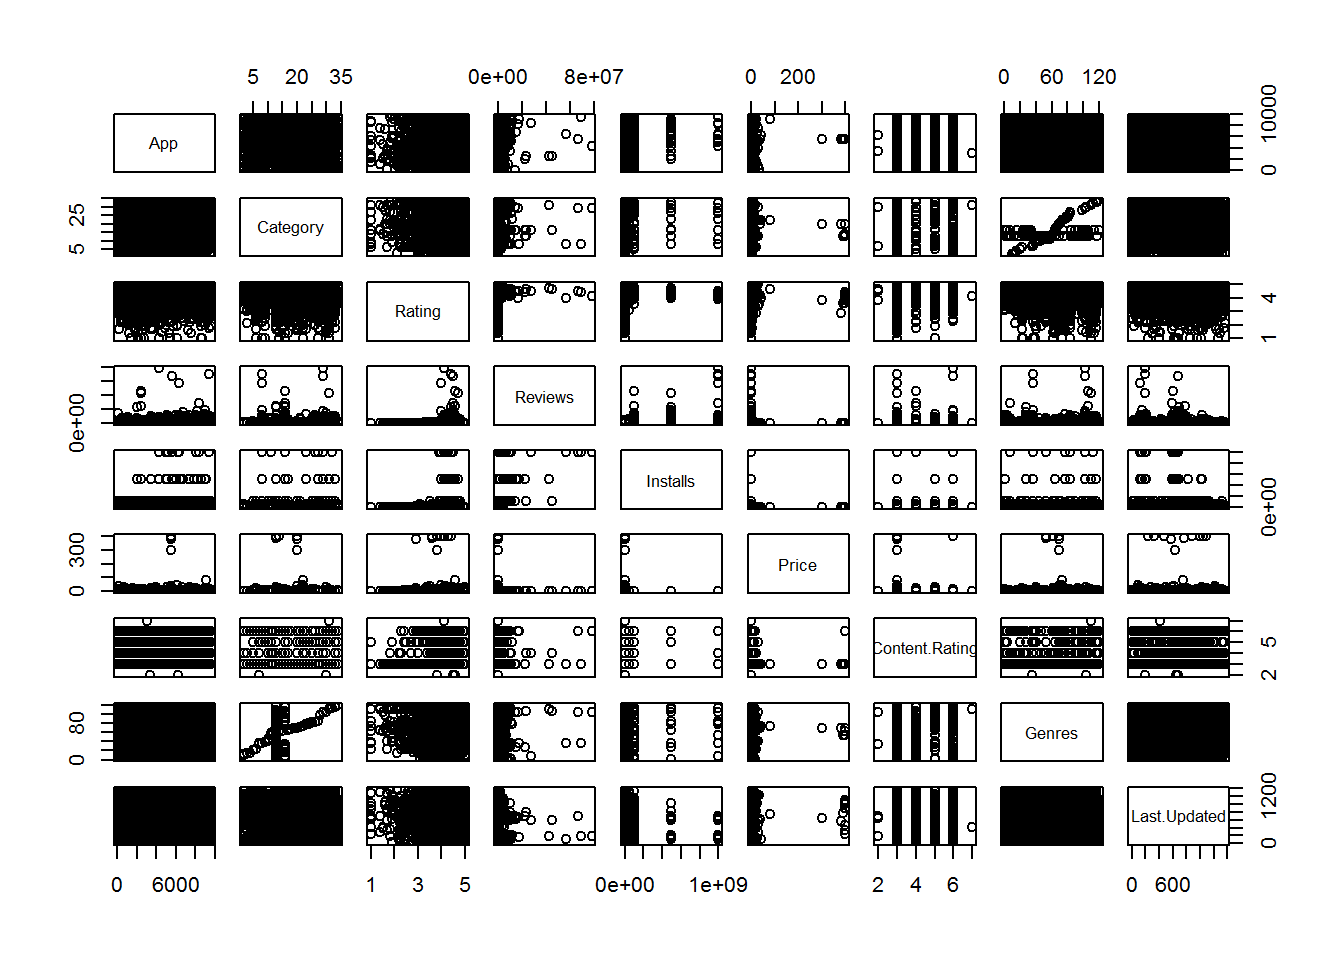
\includegraphics{Project_2_Work_files/figure-latex/unnamed-chunk-14-1.pdf}

Now, let's look at the individual variables.

\begin{Shaded}
\begin{Highlighting}[]
\KeywordTok{ggplot}\NormalTok{(Train) }\OperatorTok{+}\StringTok{ }\KeywordTok{geom_bar}\NormalTok{(}\KeywordTok{aes}\NormalTok{(}\DataTypeTok{x=}\NormalTok{Category)) }\OperatorTok{+}\StringTok{ }\KeywordTok{coord_flip}\NormalTok{()}
\end{Highlighting}
\end{Shaded}

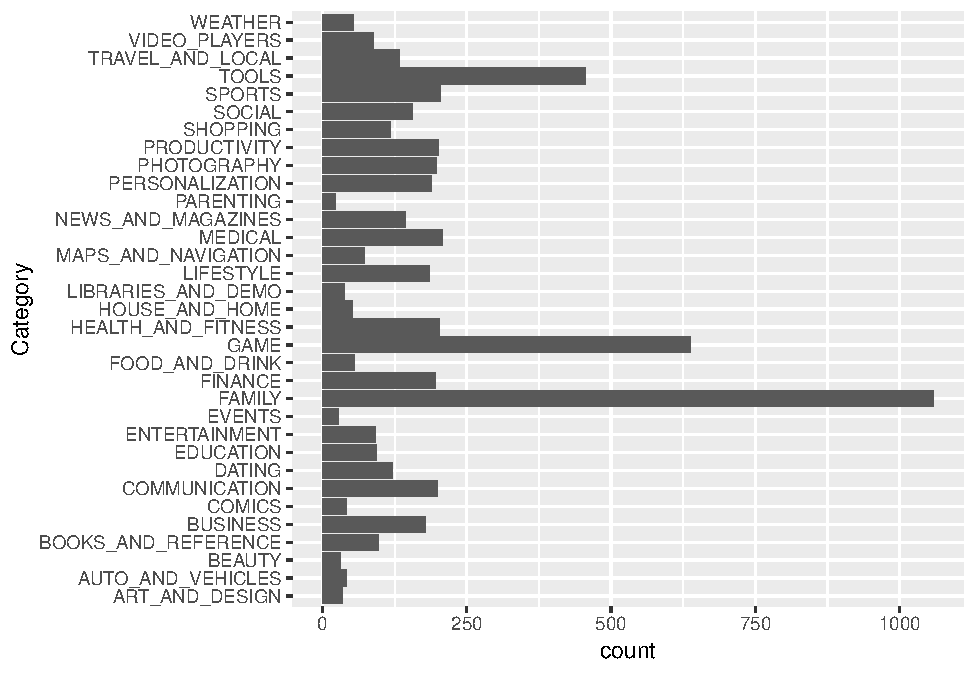
\includegraphics{Project_2_Work_files/figure-latex/unnamed-chunk-15-1.pdf}

\begin{Shaded}
\begin{Highlighting}[]
\KeywordTok{ggplot}\NormalTok{(Train) }\OperatorTok{+}\StringTok{ }\KeywordTok{geom_density}\NormalTok{(}\KeywordTok{aes}\NormalTok{(}\DataTypeTok{x=}\NormalTok{Rating),}\DataTypeTok{fill=}\StringTok{"light blue"}\NormalTok{)}
\end{Highlighting}
\end{Shaded}

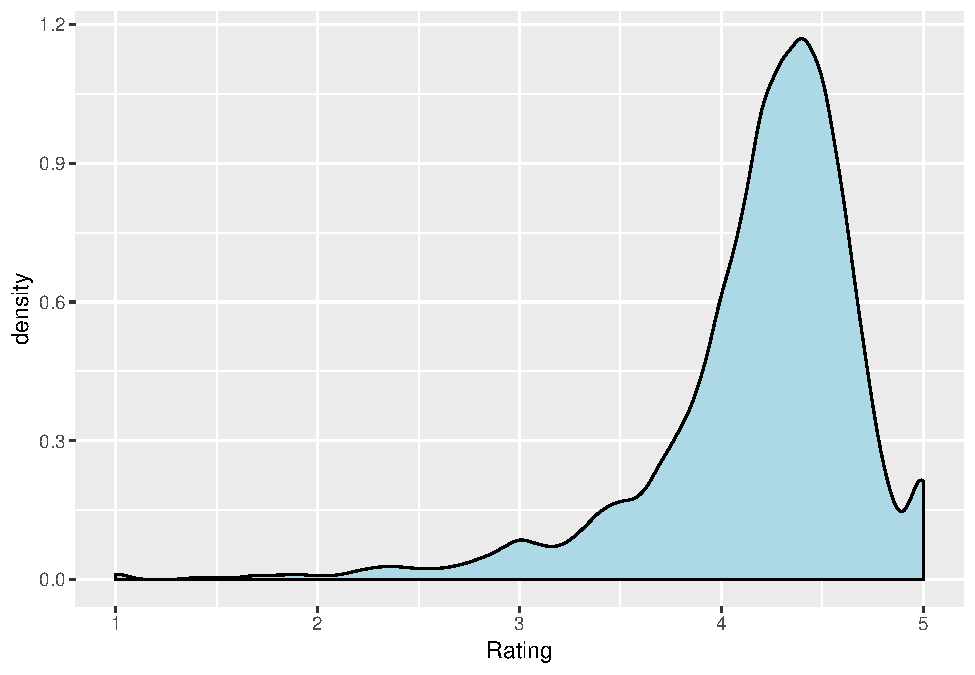
\includegraphics{Project_2_Work_files/figure-latex/unnamed-chunk-15-2.pdf}

\begin{Shaded}
\begin{Highlighting}[]
\KeywordTok{ggplot}\NormalTok{(Train) }\OperatorTok{+}\StringTok{ }\KeywordTok{geom_density}\NormalTok{(}\KeywordTok{aes}\NormalTok{(}\DataTypeTok{x=}\KeywordTok{log}\NormalTok{(Reviews)),}\DataTypeTok{fill=}\StringTok{"light green"}\NormalTok{)}
\end{Highlighting}
\end{Shaded}

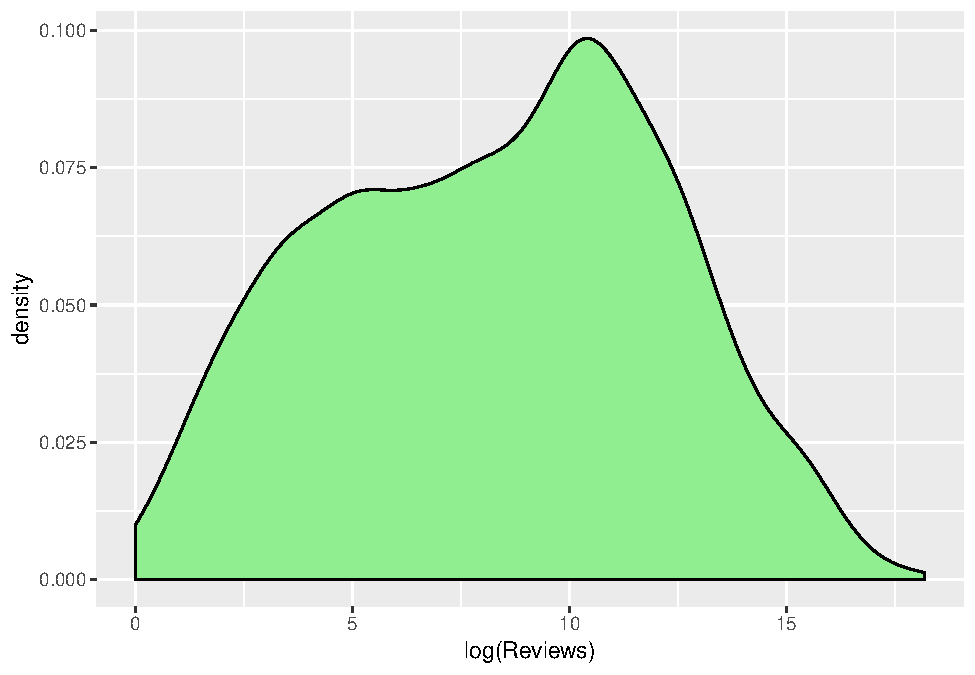
\includegraphics{Project_2_Work_files/figure-latex/unnamed-chunk-15-3.pdf}

\begin{Shaded}
\begin{Highlighting}[]
\KeywordTok{ggplot}\NormalTok{(Train) }\OperatorTok{+}\StringTok{ }\KeywordTok{geom_bar}\NormalTok{(}\KeywordTok{aes}\NormalTok{(}\DataTypeTok{x=}\KeywordTok{log}\NormalTok{(Installs)),}\DataTypeTok{fill=}\StringTok{"purple"}\NormalTok{)}
\end{Highlighting}
\end{Shaded}

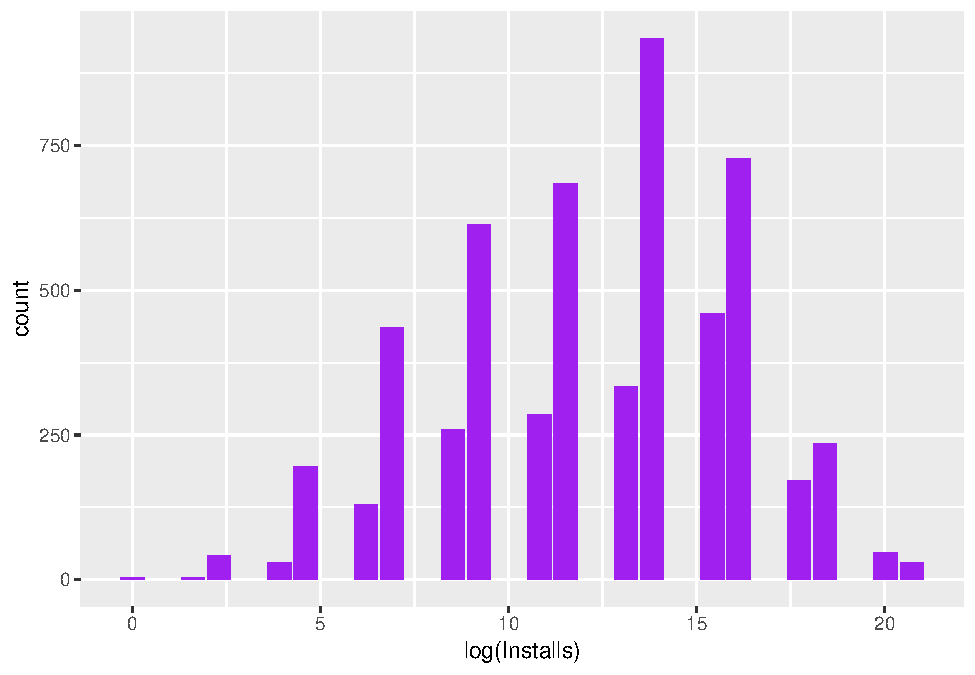
\includegraphics{Project_2_Work_files/figure-latex/unnamed-chunk-15-4.pdf}

\begin{Shaded}
\begin{Highlighting}[]
\KeywordTok{ggplot}\NormalTok{(Train) }\OperatorTok{+}\StringTok{ }\KeywordTok{geom_density}\NormalTok{(}\KeywordTok{aes}\NormalTok{(}\DataTypeTok{x=}\KeywordTok{log}\NormalTok{(Price)),}\DataTypeTok{fill=}\StringTok{"gray"}\NormalTok{)}
\end{Highlighting}
\end{Shaded}

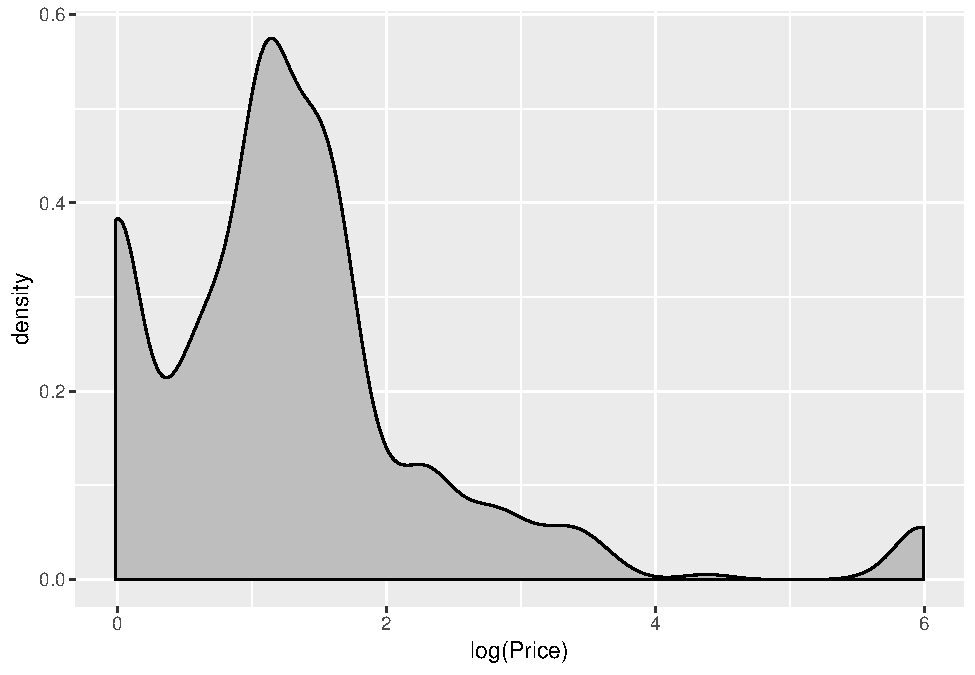
\includegraphics{Project_2_Work_files/figure-latex/unnamed-chunk-15-5.pdf}

\begin{Shaded}
\begin{Highlighting}[]
\KeywordTok{ggplot}\NormalTok{(Train) }\OperatorTok{+}\StringTok{ }\KeywordTok{geom_bar}\NormalTok{(}\KeywordTok{aes}\NormalTok{(}\DataTypeTok{x=}\NormalTok{Content.Rating)) }\OperatorTok{+}\StringTok{ }\KeywordTok{coord_flip}\NormalTok{()}
\end{Highlighting}
\end{Shaded}

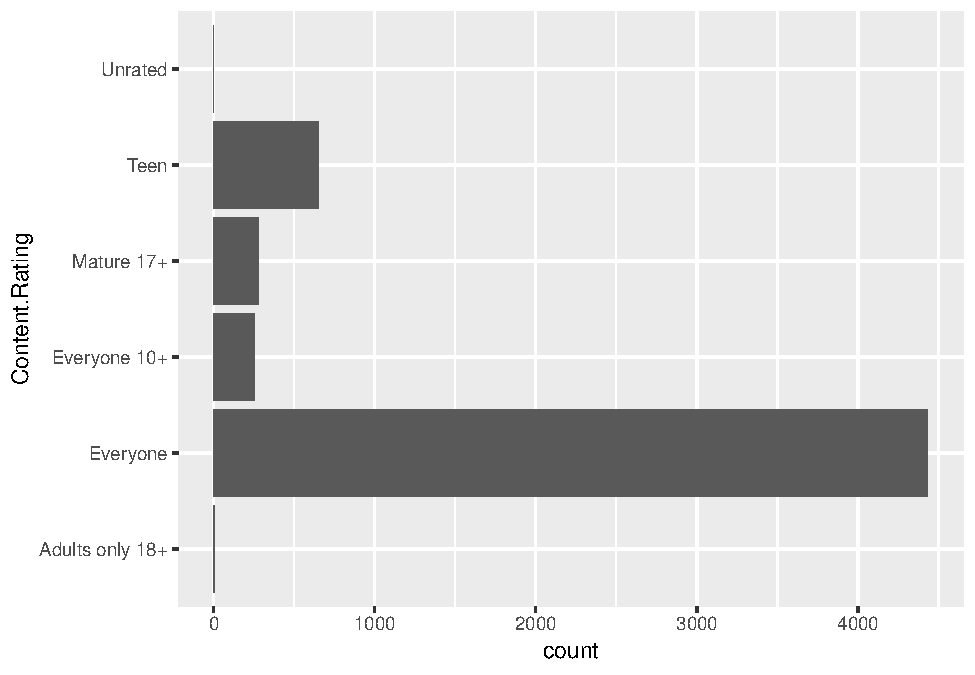
\includegraphics{Project_2_Work_files/figure-latex/unnamed-chunk-15-6.pdf}

Let's look at some of the relationships between the Rating variable, our
response, and some of the possible predictors.

\begin{Shaded}
\begin{Highlighting}[]
\KeywordTok{ggplot}\NormalTok{(Train) }\OperatorTok{+}\StringTok{ }\KeywordTok{geom_boxplot}\NormalTok{(}\KeywordTok{aes}\NormalTok{(}\DataTypeTok{x=}\NormalTok{Category,}\DataTypeTok{y=}\NormalTok{Rating), }\DataTypeTok{fill=}\StringTok{"light green"}\NormalTok{) }\OperatorTok{+}\StringTok{ }\KeywordTok{coord_flip}\NormalTok{()}
\end{Highlighting}
\end{Shaded}

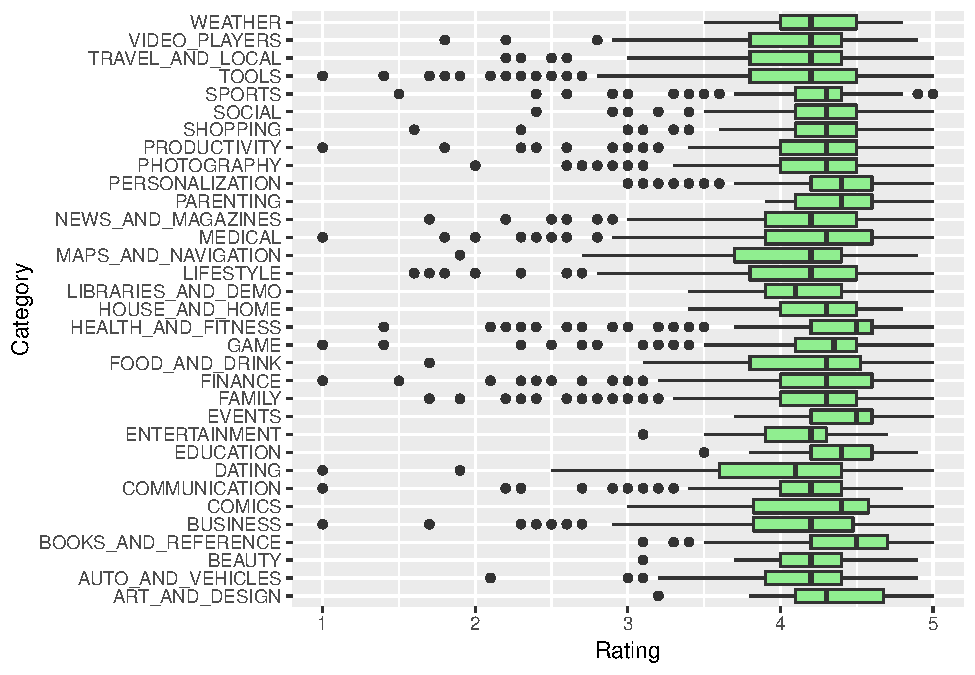
\includegraphics{Project_2_Work_files/figure-latex/unnamed-chunk-16-1.pdf}

\begin{Shaded}
\begin{Highlighting}[]
\KeywordTok{ggplot}\NormalTok{(Train) }\OperatorTok{+}\StringTok{ }\KeywordTok{geom_point}\NormalTok{(}\KeywordTok{aes}\NormalTok{(}\DataTypeTok{x=}\KeywordTok{log}\NormalTok{(Reviews),}\DataTypeTok{y=}\NormalTok{Rating), }\DataTypeTok{color=}\StringTok{"blue"}\NormalTok{)}
\end{Highlighting}
\end{Shaded}

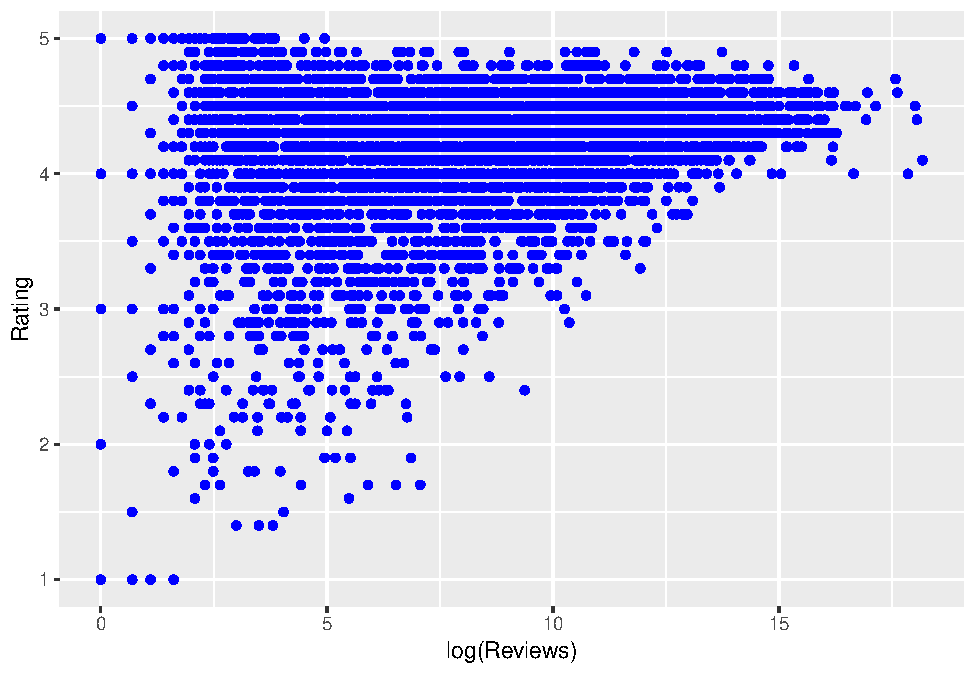
\includegraphics{Project_2_Work_files/figure-latex/unnamed-chunk-16-2.pdf}

\begin{Shaded}
\begin{Highlighting}[]
\KeywordTok{ggplot}\NormalTok{(Train) }\OperatorTok{+}\StringTok{ }\KeywordTok{geom_point}\NormalTok{(}\KeywordTok{aes}\NormalTok{(}\DataTypeTok{x=}\KeywordTok{log}\NormalTok{(Installs),}\DataTypeTok{y=}\NormalTok{Rating), }\DataTypeTok{color=}\StringTok{"purple"}\NormalTok{)}
\end{Highlighting}
\end{Shaded}

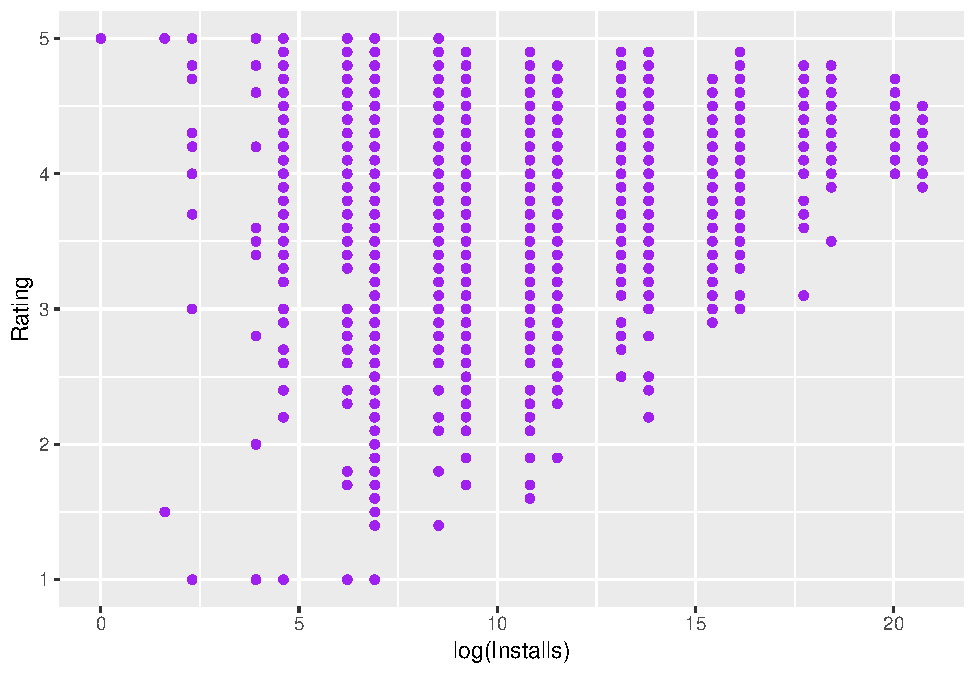
\includegraphics{Project_2_Work_files/figure-latex/unnamed-chunk-16-3.pdf}

\begin{Shaded}
\begin{Highlighting}[]
\KeywordTok{ggplot}\NormalTok{(Train) }\OperatorTok{+}\StringTok{ }\KeywordTok{geom_point}\NormalTok{(}\KeywordTok{aes}\NormalTok{(}\DataTypeTok{x=}\KeywordTok{log}\NormalTok{(Price),}\DataTypeTok{y=}\NormalTok{Rating), }\DataTypeTok{color=}\StringTok{"red"}\NormalTok{)}
\end{Highlighting}
\end{Shaded}

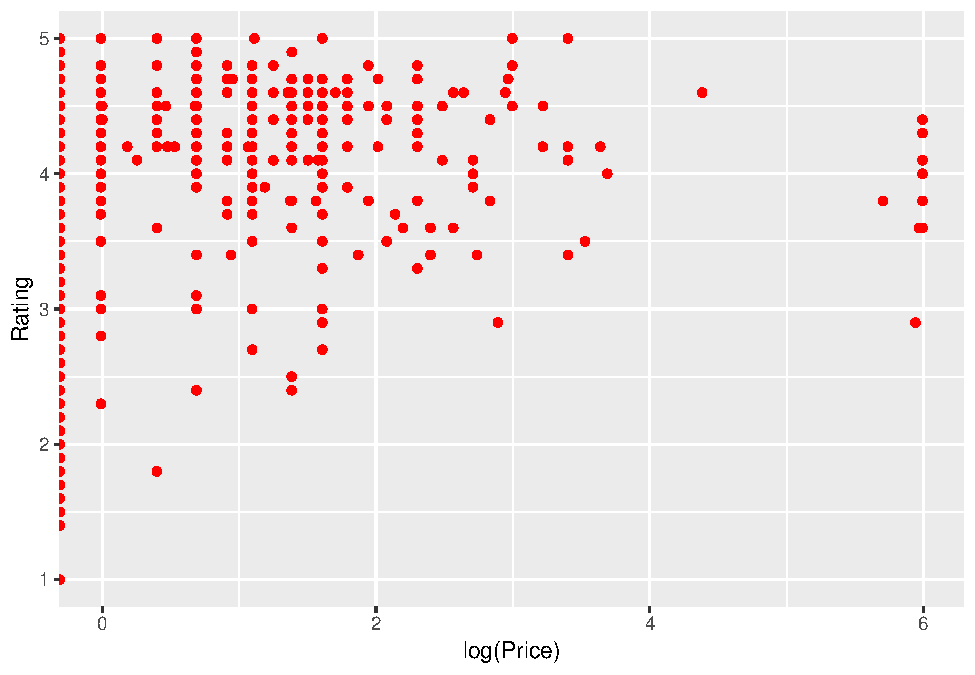
\includegraphics{Project_2_Work_files/figure-latex/unnamed-chunk-16-4.pdf}

\begin{Shaded}
\begin{Highlighting}[]
\KeywordTok{ggplot}\NormalTok{(Train) }\OperatorTok{+}\StringTok{ }\KeywordTok{geom_violin}\NormalTok{(}\KeywordTok{aes}\NormalTok{(}\DataTypeTok{x=}\NormalTok{Content.Rating,}\DataTypeTok{y=}\NormalTok{Rating), }\DataTypeTok{trim=}\OtherTok{FALSE}\NormalTok{, }\DataTypeTok{fill=}\StringTok{"light blue"}\NormalTok{)}
\end{Highlighting}
\end{Shaded}

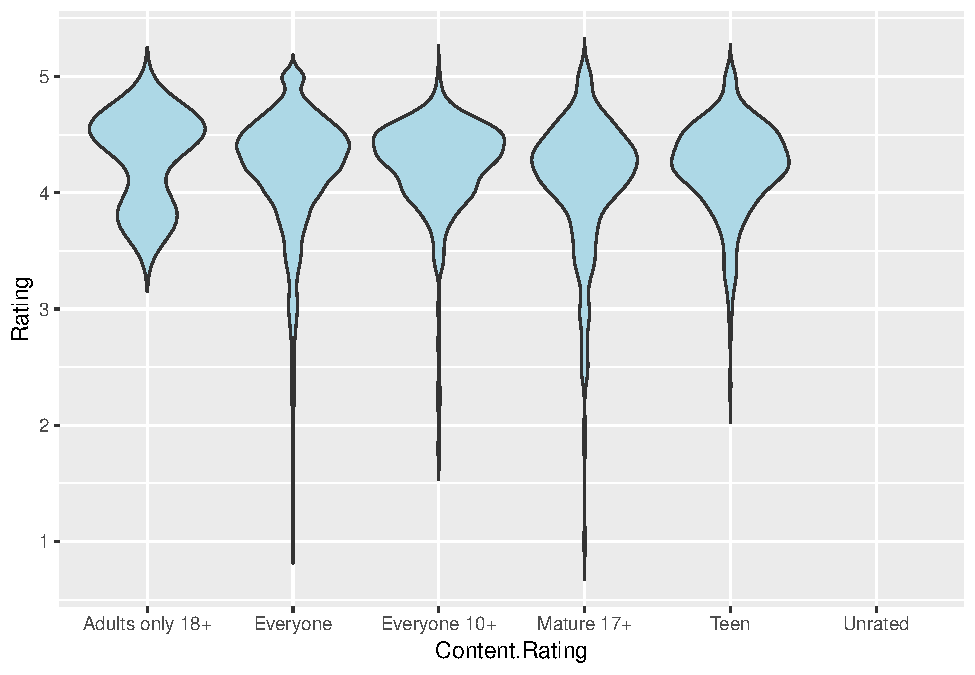
\includegraphics{Project_2_Work_files/figure-latex/unnamed-chunk-16-5.pdf}

Now, let's look at some of the relationships between the other
variables.

\begin{Shaded}
\begin{Highlighting}[]
\KeywordTok{ggplot}\NormalTok{(Train) }\OperatorTok{+}\StringTok{ }\KeywordTok{geom_boxplot}\NormalTok{(}\KeywordTok{aes}\NormalTok{(}\DataTypeTok{x=}\NormalTok{Content.Rating,}\DataTypeTok{y=}\KeywordTok{log}\NormalTok{(Installs)), }\DataTypeTok{fill=}\StringTok{"light green"}\NormalTok{)}
\end{Highlighting}
\end{Shaded}

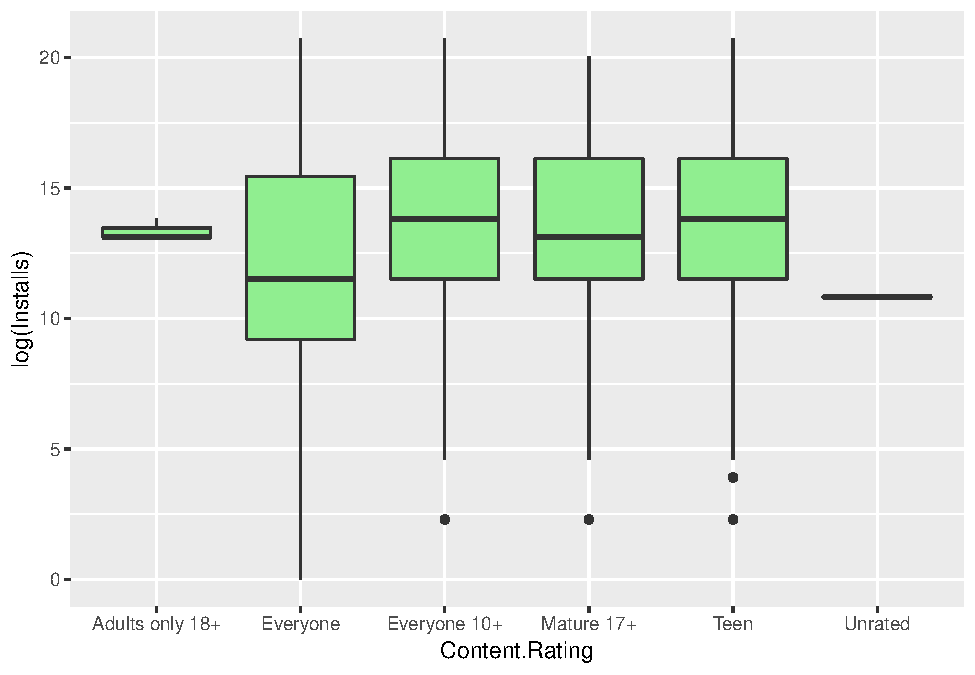
\includegraphics{Project_2_Work_files/figure-latex/unnamed-chunk-17-1.pdf}

\begin{Shaded}
\begin{Highlighting}[]
\KeywordTok{ggplot}\NormalTok{(Train) }\OperatorTok{+}\StringTok{ }\KeywordTok{geom_point}\NormalTok{(}\KeywordTok{aes}\NormalTok{(}\DataTypeTok{x=}\KeywordTok{log}\NormalTok{(Price),}\DataTypeTok{y=}\KeywordTok{log}\NormalTok{(Installs)), }\DataTypeTok{color=}\StringTok{"blue"}\NormalTok{)}
\end{Highlighting}
\end{Shaded}

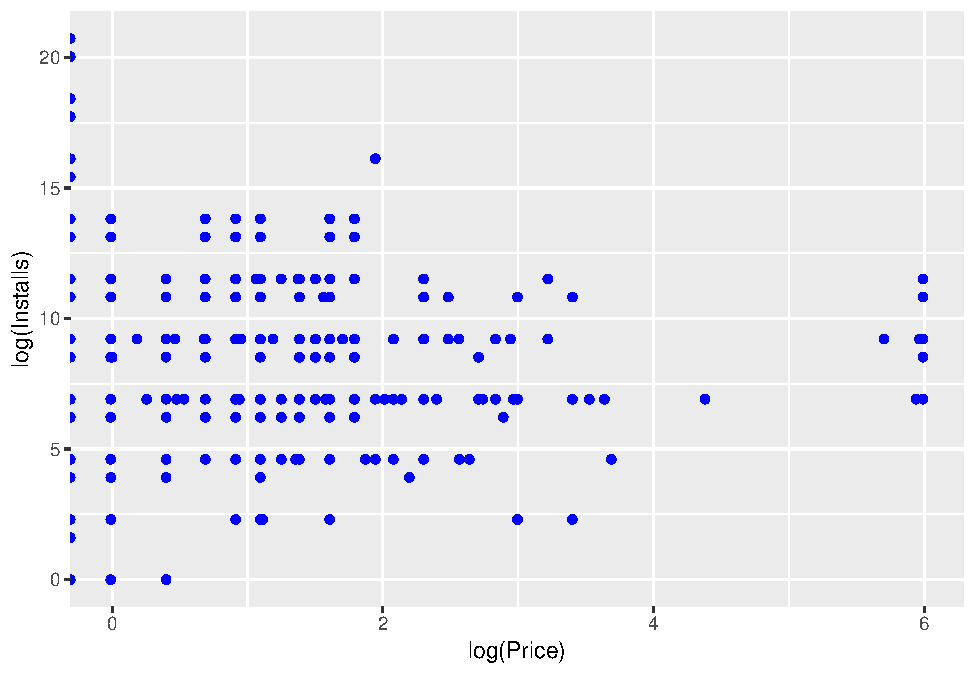
\includegraphics{Project_2_Work_files/figure-latex/unnamed-chunk-17-2.pdf}

\hypertarget{conclusion}{%
\section{Conclusion}\label{conclusion}}

It appears from the data that the Reviews variable seems quite
positively related to the Ratings variable. While ratings of 5 can be
achieved across all Review amounts, they seem to be more common with
higher Review amounts. The same can be said for the Installs variable,
in that the more installations a particular app receives could correlate
to the rating it is given. The Price appears to have essentially the
opposite effect. With the exception of free apps, lower priced apps
appear to earn higher rating scores thant more expensive apps. Content
rating does not appear to affect an app's rating.

With regard to the other relationships explored, Content Rating seemd
very equal across app installations, with apps rated as Everyone had the
most variance, probably due to the fact that most of the apps in the
data set are rated Everyone, as seen by the Content Rating bar plot
earlier. When price was compared to installations, an almost bubble
appeared in the bottom right portion of the plot, indicating that less
expensive apps might warrent more installations from users.

Moving forward, we feel that the model we are aiming to create should
include the Review, Installs, and Price variables, possibly Genres and
Category as well.

\hypertarget{questions-to-answer-in-this-study}{%
\section{Questions to Answer in This
Study}\label{questions-to-answer-in-this-study}}

\hypertarget{big-picture-question}{%
\subsection{Big Picture Question}\label{big-picture-question}}

What makes a good app?

\hypertarget{modelinghypothesis-testing}{%
\section{Modeling/Hypothesis Testing}\label{modelinghypothesis-testing}}

\hypertarget{results}{%
\section{Results}\label{results}}

\hypertarget{discussion-and-conclusions}{%
\section{Discussion and Conclusions}\label{discussion-and-conclusions}}

\hypertarget{assignment-document-words}{%
\section{Assignment Document Words}\label{assignment-document-words}}

If you are not happy with where your Project 1 ended up, you can switch
data sets; however, you will need parts I through IV for your new data
set.

Just to take a closer look at parts V through VIII:

V. Questions to answer in this study This should be a list of questions
you plan to answer in this study. Often, there is a hierarchy of
questions:

Broad questions: Interesting broad questions, but maybe not directly
addressable with adata analysis. A big question may be something like
``How biodiverse is Wildwood Park?''. Since there is no measurement of
biodiversity mentioned here, we could not possibly answer this question
directly from data, because we don't know what to measure. Narrow
questions: A narrow question will usually be a specification of a broad
question, and should indicate technical details that connect directly
with measurements we can make. For example, ``What is the alpha
diversity of avian species in Wildwood Park?'' and ``What is the beta
diversity of avian species in Wildwood Park as an area within the
central and south coast?'' In this section you should also put forward
your discussion of how you will answer these questions with models
and/or hypothesis tests.

\begin{enumerate}
\def\labelenumi{\Roman{enumi}.}
\setcounter{enumi}{5}
\item
  Modeling/Hypothesis Testing This should be your work creating models
  and running hypothesis tests. Model development should be discussed
  and included here.
\item
  Results State your (graphical, tabular and numerical) results here.
  For example, if your team has created a classification model, your
  confusion matrix should go in this section. The results should answer
  your narrow questions.
\item
  Discussion and Conclusions Discuss your results here. This is the
  point at which you can answer your broad questions by connecting them
  with your answers to your narrow questions. For example, suppose that
  we find out that several common measurements of alpha biodiversity for
  avians in Wildwood Park are high and that a common measure of beta
  diversity of avians in Wildwood Park as compared with neighboring
  regions in the central and south coast is only moderately high. Then
  we have a nuanced answer to our broad question ``How biodiverse is
  Wildwood Park?'' and this is our opportunity to discuss. You may wish
  to bring in arguments or facts from other research; if you do, make
  sure to include a works cited section and citations in your
  discussion.
\end{enumerate}

What should this slideshow and presentation look like? You and your team
will have 10 minutes to present your work using a slideshow and dialog.
Your slideshow should include information from all sections I through
VIII. The focus should be strongly on the ``important'' bits, so we
probably won't need to see the entire data dictionary in the
presentation, we'll only need to see the really tricky bits (if any) of
the data cleaning, and we'll only need to see the important bits of the
exploratory data analysis.

You should practice the usual principles of good slideshow design. We
will talk about these in class during the last few weeks.


\end{document}
